This chapter presents the tools and methods used for implementing a program for calculating the QZMIs of an image using both methods of discretization.

\section{Programming language and libraries used}
The implementation was created using the Python programming language~\cite{python} and relying on the Numpy~\cite{numpy} and Numba~\cite{numba} libraries to achieve efficient and fast computation of the moment invariants, as well as the Python Imaging Library (PIL, Pillow)~\cite{pil} for image manipulation.

Numpy provided a way to efficiently work with arrays and matrices. It also provided the quaternion package, which supports the quaternion data type.

Using the just-in-time compilation (JIT) capabilities of Numba (i.e. the \texttt{@jit} annotation), the computationally heavy parts of the implementation could be made almost as fast as native code. The disadvantage of using JIT is that it limits the available types and functions, so in the implementation the use of \texttt{@jit} is kept only to the critical, computationally intensive functions. 

\section{Calculating moments and moment invariants}
\begin{figure}[tbp]
    \centering
        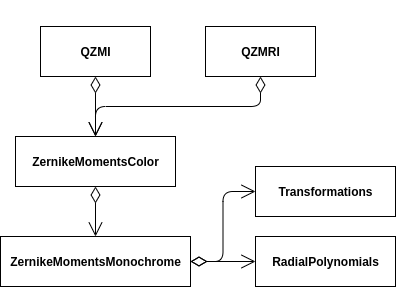
\includegraphics[width=0.5\textwidth]{figures/qzmi_classes.png}
    \caption{The relationships between the classes used to calculate QZMIs and QZMRIs}
    \label{fig:classes}
\end{figure}
To obtain the quaternion Zernike moment invariants (QZMIs) of an image as described in Section~\ref{sec:invariance}, the quaternion Zernike moments (QZMs) must be calculated first. \citeauthor{qzmi}~\cite{qzmi} showed that instead of calculating the QZMs directly by using the algebra of quaternions, it is possible to calculate the real and the imaginary parts of the quaternion-valued QZM individually by using some linear combination of the real and imaginary parts of the complex-valued, single channel Zernike moments. This means that the single channel Zernike moments have to be calculated for all three of the RGB color channels.
Furthermore, the calculation of the Zernike moments requires the computation of the radial polynomials, introduced in~\eqref{eq:radial_poly}.

To calculate the required values, the following four classes were created, each relying on the next one to perform the computation.
\begin{itemize}
    \item \texttt{QZMI}, for calculating the quaternion Zernike moment invariants
    \item \texttt{ZernikeMomentsColor}, for calculating the quaternion-valued Zernike moments
    \item \texttt{ZernikeMomentsMonochrome}, for calculating the complex-valued, single channel Zernike moments
    \item \texttt{RadialPolynomials}, for calculating the values of the radial polynomials at a given point
\end{itemize}
The relationships between these classes are shown on Figure~\ref{fig:classes}, as well as the \texttt{QZMRI} class, which calculates the rotation invariant QZMs needed for some test cases. A description of the algorithms used in these classes and the data stored by them is given below.

Since the work presented in this thesis involves changing the way an image is transformed from image coordinates to polar coordinates inside the unit circle, the classes were made modular with respect to the transformation used. This makes it easy to create and test a new image transformation function with the interface expected by the calculating classes.

\subsection{Radial polynomials}
To calculate the value of all $R_{n,m}$ radial polynomials up to some maximal degree $P$ at a point $r \in [0,1]$, the modified Kintner's method was used, as described in~\cite{kintner}. This algorithm computes the value of $R_{n,m}(r)$ for all $0 \leq |m| \leq n \leq P$, ($n - |m|$ is even) with complexity $\mathcal{O}(N^2)$. This method is ideal for the computation of all radial polynomial values up to a maximum degree.

Since this method is called many times during the calculation of Zernike moments, just-in-time compilation was used to further increase efficiency. Figure~\ref{fig:radial_code} shows the JIT-enabled function.

\begin{figure}[tbp]
    \centering
    \begin{lstlisting}[language=Python]
@jit(void(float64, int32, float64[:,:]), nopython=True)
def calculateRadialPolynomials(r, P, values):
  values[0,0] = 1
  values[1,1] = r
  for n in range(2,P + 1):
    h = n*(n - 1)*(n - 2)
    K2 = 2*h
    values[n,n] = (r**n)
    values[n,n-2] = n*values[n,n] - (n-1)*values[n-2,n-2]
    for m in range(n-4,-1,-2):			
      K1 = (n + m)*(n - m)*(n - 2)/2
      K3 = (-1)*m*m*(n - 1) - h
      K4 = (-1)*n*(n + m - 2)*(n - m - 2)/2
      r2 = r**2
      values[n,m] = ((K2*r2+K3)*values[n-2,m]+K4*values[n-4,m])/K1\end{lstlisting}
    \caption{Function for calculating radial polynomial values}
    \label{fig:radial_code}
\end{figure}

\subsection{Complex Zernike moments}
The \texttt{ZernikeMomentsMonochrome} class calculates the conventional Zernike moments of degree at most $P$ of a square $N \times N$, single channel (grayscale) image. The algorithm is based directly on the discretized definition of the Zernike moments.
For the original linear transformation of the image onto the unit disk, this gives:
\begin{gather*}
    \begin{split}
    Z_{n,m}(f) &= \lambda\frac{(n+1)}{(N-1)^2}\sum_{x=1}^{N}\sum_{y=1}^{N}f(x,y)V_{n,m}^{*}(r_{x,y},\theta_{x,y}) \\
    &= \lambda\frac{(n+1)}{(N-1)^2}\sum_{x=1}^{N}\sum_{y=1}^{N}f(x,y)R_{n,m}(r_{x,y})e^{-\bm{i}m\theta_{x,y}} \\
    &= \lambda\frac{(n+1)}{(N-1)^2}\sum_{x=1}^{N}\sum_{y=1}^{N}f(x,y)R_{n,m}(r_{x,y})(\cos (m\theta_{x,y}) - \bm{i}\sin (m\theta_{x,y})),
    \end{split}
\end{gather*}
where $0\leq |m| \leq n \leq P$, $n - |m|$ is even, $(r_{x,y},\theta_{x,y})$ are the $(x,y)$ coordinates transformed to the unit disk, $\lambda$ is the scaling parameter also given by the transformation (as described in Section~\ref{sec:discretization}) and $f$ is the real-valued, grayscale image.

By precomputing the sin and cos values for all possible $m$ and $\theta_{x,y}$ values, as well as the values of the radial polynomials, this formula gives an efficient way of calculating the real and imaginary parts of the Zernike moments separately. This way only primitive data types have to be used during the computation and it can be made more efficient using JIT.

Also, there is no need to calculate the Zernike moments for negative $m$ values, as the $Z_{n,m}(f) = Z_{n,-m}(f)^{*}$ identity can be used later to obtain those values.

\subsection{Quaternion Zernike moments}
The class \texttt{ZernikeMomentsColor} calculates the quaternion Zernike moments of an RGB image. First, the conventional Zernike moments for each of the three color channels are calculated, then the relationship between QZMs and Zernike moments is used to construct the quaternions~\cite{qzmi}.
\begin{gather*}
    \begin{split}
        Z_{n,m}^R(f) = &-\frac{1}{\sqrt{3}}\left( \ip(Z_{n,m}(f_R)) + \ip(Z_{n,m}(f_G)) + \ip(Z_{n,m}(f_B)) \right)\\
        &+\left[\rp(Z_{n,m}(f_R)) + \frac{1}{\sqrt{3}}\left(\ip(Z_{n,m}(f_G)) - \ip(Z_{n,m}(f_B))\right)\right]\bm{i}\\
        &+\left[\rp(Z_{n,m}(f_G)) + \frac{1}{\sqrt{3}}\left(\ip(Z_{n,m}(f_B)) - \ip(Z_{n,m}(f_R))\right)\right]\bm{j}\\
        &+\left[\rp(Z_{n,m}(f_B)) + \frac{1}{\sqrt{3}}\left(\ip(Z_{n,m}(f_R)) - \ip(Z_{n,m}(f_G))\right)\right]\bm{k},\\
    \end{split}
\end{gather*}
where $f$ is an RGB image and $f_R, f_G, f_B$ are the red, green and blue color channels respectively.

Again, only the QZMs $Z_{n,m}^R$ ($m \geq 0$) are calculated, because for $m < 0$ the $Z_{n,m}^R(f) = Z_{n,-m}^R(f)^{*}$ equality can be used.

\subsection{Invariants}
The class \texttt{QZMI} is responsible for computing the combined rotation, scaling and translation (RST) invariant moments, while the class \texttt{QZMRI} computes the moments which are invariant only to rotation.
The invariants for scaling and rotation are calculated directly using the QZMs, based on the formulas described in Section~\ref{sec:invariance}.

To achieve translation invariance, the common centroid of the RGB image is calculated based on the formulas described by ~\citeauthor{affine_color}~\cite{affine_color}.
\begin{gather*}
    \left\{x_c,y_c\right\} = \left\{\frac{M_{10}(f_R)+M_{10}(f_G)+M_{10}(f_B)}{M_{00}(f_R)+M_{00}(f_G)+M_{00}(f_B)}, \frac{M_{01}(f_R)+M_{01}(f_G)+M_{01}(f_B)}{M_{00}(f_R)+M_{00}(f_G)+M_{00}(f_B)}\right\},
\end{gather*}
where $f_R, f_G, f_B$ are the grayscale images corresponding to the red, green and blue color channels respectively, and $M_{10}, M_{01}, M_{00}$ are the regular image moments introduced in~\eqref{eq:regular_moment}.
The original image $f$ is then translated in image coordinates such that the origin falls on the common centroid $\{x_c,y_c\}$, and the other invariants are then calculated based on this translated image.


\section{New image transformation}\label{sec:new_trans}
The new image transformation, as described in Chapter~\ref{sec:maths}, requires the calculation of the roots of the $n^{th}$ degree Legendre polynomials $P_n$, as well as calculating the integrals of the Lagrange basis polynomials over the roots of $P_n$. Furthermore, since when applying the linear transformation from image coordinates to polar coordinates, the pixels of the image do not fall exactly on any point in the new discrete points system, other interpolating methods have to be used to approximate the image values at these points.

Because of the modularity of the previously described classes, it is possible to swap the old transformation to the new one. With some minor modifications during the calculation of the conventional Zernike moments because of the new discretization formula containing a different measure, %TODO: ref equation
the previous classes can be used to obtain the QZMIs using the new method of discretization.

\subsection{Roots of Legendre polynomials}
The roots of the Legendre polynomial $P_n$ are essential for the calculation of the new points system. An explicit formula, which gives the roots does not exist, thus an efficient and fast iterative algorithm is needed to calculate these roots.

The $n^{th}$ degree Legendre polynomial $P_n$ satisfies the following differential equation:
\begin{gather}
    (1-x^2)P_n''(x) - 2xP_n'(x) + n(n+1)P_n(x) = 0.\label{eq:legendre_de}
\end{gather}
A fast algorithm for calculating the roots of $P_n$, based on this differential equation was presented by \citeauthor{legendre_algo}~\cite{legendre_algo}. The algorithm uses a second-order Runge-Kutta method (namely the midpoint method) to solve the Prüfer-transformed version of~\eqref{eq:legendre_de} for some given initial condition. A first approximation for a root of $P_n$ can be obtained from the solution of the initial value problem. This approximation is then further refined by Newton's method.
Subsequent roots can be calculated using the same method but starting from different initial conditions defined by the previous root.

In practice, this algorithm calculates the roots of $P_n$ with accuracy up to machine precision in only a fix, limited number of iterations for both the Runge-Kutta and the Newton's method.

\subsection{Computing the discrete measure}
To calculate the Zernike moments over the discrete orthogonal points system, instead of the $\lambda$ scaling factor used in the linear transformation, a different measure is used. To calculate this $\mu_{k,N}$ measure (defined in% TODO: keplet hivatkozni, jeloles egyeztetni
), the following integral has to be calculated:
\begin{gather*}
    \mathcal{A}_{k,N} = \int_{-1}^{1}\ell_{k,N}(x)\dif x,
\end{gather*}
where $\ell_{k,N}$ is the $k^{th}$ Lagrange basis polynomial corresponding to the roots of the Legendre polynomial $P_N$.

The Gauss-Legendre quadrature is based on the roots of the Legendre polynomial $P_n$ of degree $n$. Let $x_1,x_2,\ldots,x_n$ be the roots of $P_n$.
\begin{gather*}
    \int_{-1}^{1}f(x)\dif x \approx \sum_{k=1}^n w_k f(x_k), \\
    w_k = \frac{2}{(1-x_k^2)(P_n'(x_k))^2}.
\end{gather*}
The quadrature is exact for all polynomials whose degree is at most $2n-1$. Now $\ell_{k,N}(x)$ is an $N-1$ degree polynomial, so the Gauss-Legendre quadrature with $n=N$ is exact for $\ell_{k,N}$. Furthermore, $\ell_{k,N}$ is defined such that $\ell_{k,N}(x_i) = 0$ for $i \neq k$, and $\ell_{k,N}(x_k) = 1$ Thus:
\begin{gather*}
    \int_{-1}^{1}\ell_{k,N}(x)\dif x = w_k = \frac{2}{(1-x_k^2)(P_n'(x_k))^2}.
\end{gather*}

Since the roots of the Legendre polynomial $P_N$ must be computed to obtain the points system, this formula gives an easy and fast way to calculate the exact values of $\mu_{k,N}$.

\subsection{Image interpolation}
After obtaining the discrete orthogonal points system the values of the image function have to be approximated at each point, because the original pixel values do not fall exactly on the new points. Now we describe some reasonable ways of resampling the image data to fit these new points.

First, the image is linearly transformed onto the unit disk using the transformation shown on Figure~\ref{fig:transform2}, so that the the transformed image covers the entire unit disk. This transformation is used as opposed to the one on Figure~\ref{fig:transform1}, because the points system covers the entire unit disk, so the image also has to cover the whole disk.

There are two ways to approximate the values at each point, depending on the number of points in the discrete orthogonal points system.

\begin{figure}[tb]
    \centering
    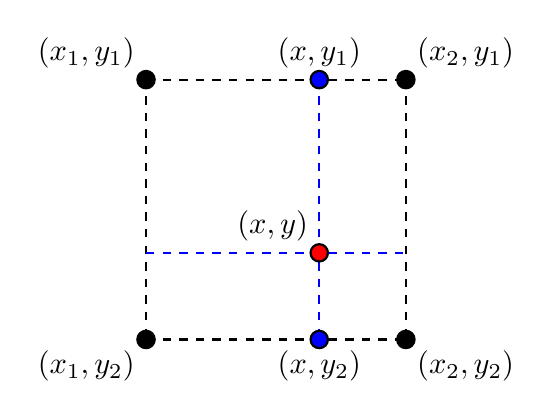
\begin{tikzpicture}[thick,scale=1.1, every node/.style={transform shape}]
        \draw[thick,dashed] (-2,2) -- (1,2);
        \draw[thick,dashed] (-2,2) -- (-2,-1);
        \draw[thick,dashed] (1,2) -- (1,-1);
        \draw[thick,dashed] (-2,-1) -- (1,-1);
        \draw[fill] (-2,2) circle (0.1) node[anchor=south east] {$(x_1,y_1)$};
        \draw[fill] (1,2) circle (0.1) node[anchor=south west] {$(x_2,y_1)$};
        \draw[fill] (-2,-1) circle (0.1) node[anchor=north east] {$(x_1,y_2)$};
        \draw[fill] (1,-1) circle (0.1) node[anchor=north west] {$(x_2,y_2)$};
        
        \draw[thick,blue,dashed] (0,2) -- (0,-1);
        \draw[thick,blue,dashed] (-2,0) -- (1,0);
        \draw[fill=red] (0,0) circle (0.1) node[anchor=south east] {$(x,y)$};
        \draw[fill=blue] (0,2) circle (0.1) node[anchor=south] {$(x,y_1)$};
        \draw[fill=blue] (0,-1) circle (0.1) node[anchor=north] {$(x,y_2)$};
    \end{tikzpicture}

    \caption{The point $(x,y)$ and its neighboring points, which are used to approximate $f(x,y)$ by bilinear interpolation}
    \label{fig:bilinear}
\end{figure}

\paragraph{Approximately the same number of points as pixels.}
If the number of points is approximately the same as the number of pixels in the image, then bilinear interpolation can be used for each point.

First, the four pixels of the image that are closest to the given point $(x,y)$ are determined. These four points form a square. Then, the weighted average of these points is calculated along the $x$ axis, giving approximate function values at two points, which only differ in their $y$ coordinate. Finally, the weighted average of the function values at these points is calculated to get the approximation of $f(x,y)$. The points involved in this interpolation are shown on Figure~\ref{fig:bilinear}.



\paragraph{Much less points than the number of pixels.}
If the number of points is far less than the number of pixels, then using bilinear interpolation many of the original pixel values would not be represented in the final approximate function values. Therefore, the following algorithm is used to approximate function values using discrete integration.

First, for each pixel in the original image, determine which point it falls closest to after the linear transformation. Then, for each point in the discrete orthogonal points system, calculate the average of the pixels that are closest to that point. This algorithm divides the unit disk into annular sections based on the proximity to the new points. This is shown on Figure~\ref{fig:interpolation_integral}.

\begin{figure}[tb]
    \begin{subfigure}{.45\textwidth}
    \centering
    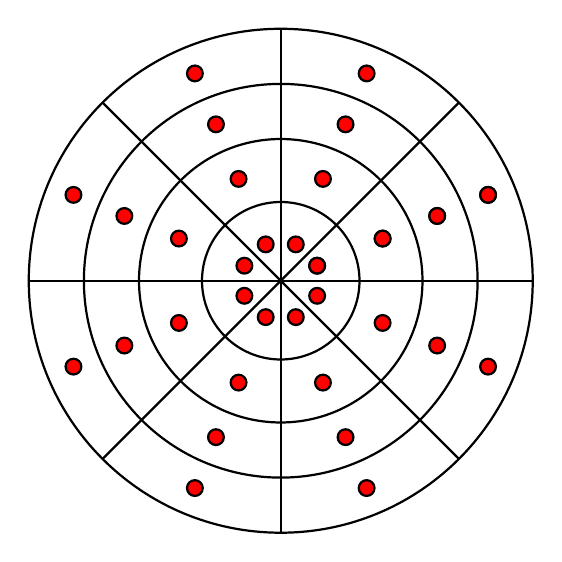
\begin{tikzpicture}[thick,scale=1, every node/.style={transform shape}]
        \foreach \r in {1,1.8,2.5,3.2}
            \draw (0,0) circle (\r);
        \foreach \x in {0,45,...,360} {
            \draw[thick] (0,0) -- (\x:3.2);
            \foreach \r in {0.5,1.4,2.15,2.85}
                \draw[fill=red] (22.5+\x:\r) circle (0.1);
        }
    \end{tikzpicture}

    \caption{The points system on the unit disk and the annular sectors over which the pixel values are averaged.}
    \end{subfigure}
    \hspace{.05\textwidth}
    \begin{subfigure}{.45\textwidth}
        \centering
        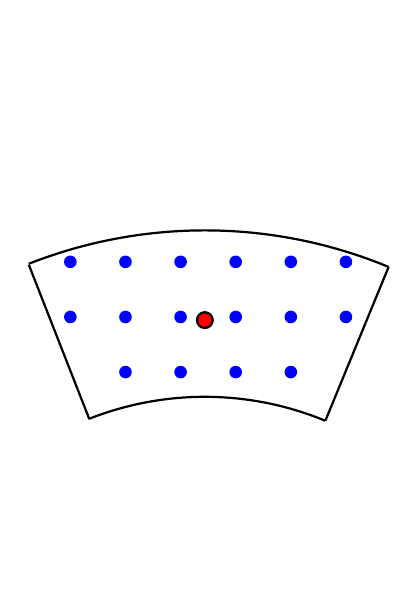
\begin{tikzpicture}[thick,scale=1, every node/.style={transform shape}]
            \draw (6.1*0.3826,6.1*0.9304) arc (67.5:111.5:6.1);
            \draw (4*0.3826,4*0.9304) arc (67.5:111.5:4);
            \draw (4*0.3826,4*0.9304) -- (6.1*0.3826,6.1*0.9304);
            \draw (-4*0.3665,4*0.935) -- (-6.1*0.3665,6.1*0.935);
            \foreach \x in {0,1,...,3} {
                \foreach \y in {2,3,...,4} {
                    \fill[color=blue] (0.7*\x-0.7*1.44,0.7*\y+0.7*4.2) circle (0.08);
                }
            }
            \fill[color=blue] (-0.7-0.7*1.44,0.7*3+0.7*4.2) circle (0.08);
            \fill[color=blue] (-0.7-0.7*1.44,0.7*4+0.7*4.2) circle (0.08);
            \fill[color=blue] (4*0.7-0.7*1.44,0.7*3+0.7*4.2) circle (0.08);
            \fill[color=blue] (4*0.7-0.7*1.44,0.7*4+0.7*4.2) circle (0.08);
            \draw[fill=red] (90:5) circle (0.1);
            \draw[color=white] (0,2) circle (0.1);
            \draw[color=white] (0,8.60) circle (0.1);
        \end{tikzpicture}
    
        \caption{A single annular sector with the original image pixels (blue) and the point in which the approximate function value has to be calculated (red).}
        \end{subfigure}
        \caption{}
    \label{fig:interpolation_integral}
\end{figure}

The comparison between one of the original transformations and the two methods for approximating function values is shown on Figure~\ref{fig:pepper_trans} on the peppers image from the USC-SIPI Image Database~\cite{usc_sipi}.

\begin{figure}
    \begin{subfigure}{.49\textwidth}
        \centering
    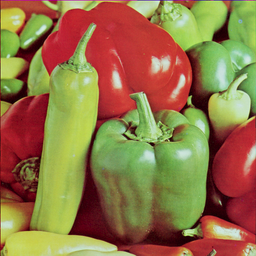
\includegraphics[width=\textwidth]{figures/pepper_color_256.png}
    \caption{Original image}
    \end{subfigure}
    \begin{subfigure}{.49\textwidth}
        \centering
    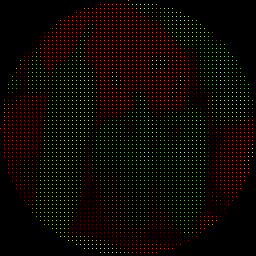
\includegraphics[width=\textwidth]{figures/pepper_square.png}
    \caption{Original transformation}
    \end{subfigure}
    \begin{subfigure}{.49\textwidth}
        \centering
    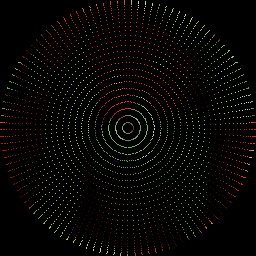
\includegraphics[width=\textwidth]{figures/pepper_bilinear.png}
    \caption{Bilinear interpolation}
    \end{subfigure}
    \begin{subfigure}{.49\textwidth}
        \centering
    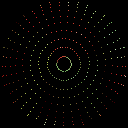
\includegraphics[width=\textwidth]{figures/pepper_integral.png}
    \caption{Interpolation by integrals}
    \end{subfigure}
    \caption{Different transformations with different interpolation methods of the peppers image.}
    \label{fig:pepper_trans}
\end{figure}